\documentclass[12pt]{article}

\usepackage[preprint]{neurips_2021}

\usepackage[utf8]{inputenc} % allow utf-8 input
\usepackage[T1]{fontenc}    % use 8-bit T1 fonts
\usepackage{hyperref}       % hyperlinks
\usepackage{url}            % simple URL typesetting
\usepackage{booktabs}       % professional-quality tables
\usepackage{amsfonts}       % blackboard math symbols
\usepackage{nicefrac}       % compact symbols for 1/2, etc.
\usepackage{microtype}      % microtypography
\usepackage{xcolor}

\usepackage{amsmath}

\usepackage{graphicx}

\graphicspath{ {./images/} }

\usepackage{amsthm}
\newtheorem{definition}{Definition}

\newcommand{\contentdescription}[1]{}

\newcommand{\TODO}[2]{{#2}}

\title{Report}

\author{
    Pavlo Melnyk \\
    \texttt{pavlo.melnyk@liu.se} \\
    \And
    Julian Alfredo Mendez \\
    \texttt{julian.mendez@umu.se} \\
    \And
    Emanuel S\'{a}nchez Aimar \\
    \texttt{emanuel.sanchez.aimar@liu.se} \\
}

\begin{document}

    \maketitle

    \begin{abstract}
        \contentdescription{
            Abstract (5-10\%):
            Give an overview of what you have done in the project with the key results and findings of your work.
            Should be no more than 300 words.
        }

        Recognition and representation of 3D data is a challenging and fruitful topic.
        In this paper, we analyzed the studies considered in~\cite{pmlr-v80-achlioptas18a}, and re-implemented their approach using PyTorch\footnote{https://pytorch.org}.

        They introduced a deep AutoEncoder (AE) network that has ``state-of-the-art reconstruction quality and generalization ability''.
        Their representations can outperform methods on 3D recognition tasks and let editing using algebraic manipulations.

        They perform studies of GANs operating on the raw point clouds, GANs trained with the AEs.
    \end{abstract}


    \section{Introduction}

    \contentdescription{
        Introduction (5-15\%):
        Describe the problem, the approach of the paper, the experiments, and the results.
        At the high-level talk about what you worked on in your project and why it is important.
        Then give an overview of your results.
    }

    The applications of representing three-dimensional (3D) images are numerous, like its use in augmented and virtual reality.
    In turn, these can be applied on a variety of domains, ranging from medicine to gaming.

    One of the critical problems of 3D sampling is the different rotations an image can have.

    We applied three approaches: raw-GAN, autoencoder, and $l$-GAN, which are defined in the subsequent sections.

    This report is about a reimplementation of~\cite{pmlr-v80-achlioptas18a} using PyTorch.


    \section{Related Work}
    \contentdescription{
        Related Work (5-15\%):
        Discuss the published work related to your project paper, the types of experiments you do and the additional method that you have added to this work or you have compared this paper with (if any).
    }

    Some the relevant related work we can mention is described in~\cite{arxiv:1612.00593}.

    The architectures used in that paper is based on AutoEncoders (AEs)\cite{doi:10.5555/65669.104451}\cite{arxiv:1312.6114},
    and Gnerative Adversarial Networks (GANs)\cite{NIPS2014_5ca3e9b1}\cite{arxiv:1511.06434}\cite{arxiv:1612.02136},
    and were used to generate samples from complex underlying distributions.


    \section{Methods}
    \contentdescription{
        Methods (15-25\%):
        Describe the original paper's method to the extent that you would need to make your report and findings understandable.
        Otherwise, here you can describe other methods that you compare with or other methods that you apply on top of what you reimplemented.
        Here, you also try to justify any methodical modification or incremental changes that you have added to the original paper.
        It may be helpful to include figures, diagrams, or tables to describe your method or compare it with other methods.
    }

    \begin{definition}
        A \emph{point cloud} is a set of points $(x, y, z)$ in a Euclidean coordinate frame.
    \end{definition}

    In this paper, a point cloud usually represents a surface.

    \begin{definition}
        A \emph{metric} or \emph{distance function} is a function defined
        $d: X \times X \to \mathbb{R}_{\geq 0}$
        with the following properties:

        \begin{enumerate}
            \item $d(x,y) = 0 \Leftrightarrow x = y$
            \item $d(x,y) = d(y,x)$
            \item $d(x,y) \leq d(x,z) + d(z,y)$
        \end{enumerate}

        A \emph{pseudo-distance} is like a distance, but it allows different points to have distance 0, and the first requirement is replaced by:
        \[d(x,x) = 0\]
    \end{definition}

    \begin{definition}
        The \emph{Earth Mover's distance (EMD)}~\cite{doi:10.1023/A:1026543900054} for two equally sized $S_{1}$, $S_{2}$, $S_{1} \subseteq \mathbb{R} ^{3}$ and $S_{2} \subseteq \mathbb{R} ^{3}$, $\Phi = \{ \phi \mid \phi: S_{1} \to S_{2} \land \phi \text{ is a bijection}\}$ is

        \[d_{EMD}(S_{1}, S_{2}) = \min _{\phi \in \Phi} \sum_{x \in S_{1}} || x - \phi(x)||_{2}\]
    \end{definition}

    \begin{definition}
        The \emph{Chamfer (pseudo)-distance (CD)} is defined as follows:

        \[d_{CD}(S_{1}, S_{2}) = \sum_{x \in S_{1}} \min _{y \in S_{2}} || x - y||_{2}^{2} +
        \sum_{y \in S_{2}} \min_{x \in S_{1}} ||x - y||_{2}^{2}\]
    \end{definition}

    The EMD and the CD are used to measure the sampling error of the results.

    \begin{definition}
        The \emph{autoencoder} architecture is a design to reproduce its input, and is composed by an \emph{encoder} (E) and a \emph{decoder} (D).

        The encoder takes an input $x$ and produces a compressed version $z$, which is called the \emph{latent representation} of $x$. The decoder tries to reconstruct $x$ by using $z$ as input, and returns $\hat{x}$ as output.

        The whole pipeline can be represented by:
        \[x \to E \to z \to D \to \hat{x}\]
    \end{definition}

    The basic architecture used in this paper is the Generative Adversarial Networks (GANs).

    \begin{definition}
        A \emph{Generative Adversarial Network} (GAN) is an interplay between a \emph{generator} (G) and a \emph{discriminator} (D).
        In that interaction, the generator tries to synthesize samples that mimic real data by giving a randomly created sample through the generator function, while the discriminator needs to distinguish the synthesized examples from the real ones.
    \end{definition}

    \begin{definition}
        Given two sets of point clouds $A$ and $B$, and given a distance, either CD or EMD, we say that \emph{coverage} is a measure for the fraction of the point clouds in $B$ that were matched to point clouds in $A$, such that each point cloud in $A$ is related to its the closest neighbor in $B$ using the given distance.
    \end{definition}

    \begin{definition}
        We define the \emph{fidelity} of $A$ with respect to $B$ as the \emph{minimum matching distance} (MMD) of matching each point in $B$ to a point in $A$.
        The \emph{MMD} is computed as an average of the individual point-wise distances, using either the CD or EMD.
        They are called the \emph{MMD-CD} and \emph{MMD-EMD} respectively.
    \end{definition}

    Fidelity and coverage are meant to measure the global error of the computation.

    Let us see an intuitive example behind fidelity and the MMD.
    If we sample chairs, we can look at the closest matching chair from the generated ones for a given metric.


    \section{Data, experiments and findings}
    \contentdescription{
        Data, experiments and findings (30-40\%):
        Describe the data you are working with for your project.
        What type of data is it?
        Where did it come from?
        How much data are you working with?
        Did you have to do any preprocessing, filtering, or other special treatment to use this data in your project?
        Describe and present the experiments that you performed and what is the reason for those experiments.
        Where applicable define evaluation metrics that you used. Discuss the results that you got.
    }

    We can describe our experiments using 3 stages.

    \textbf{Stage 1}
    We trained our encoder (E) as defined in the definition of autoencoder.
    In the bottleneck, $z$ represents the compressed representation.
    For comparison, in the raw-GAN approach, a point cloud is used instead of a compressed representation.

    \textbf{Stage 2}
    We sampled using a Gaussian distribution $\mathcal{N}(0,\sigma)$.

    \textbf{Stage 3}
    This is used to sample and create using GANs
    $C' = \sigma(z)$
    $P = D(C')$

    We used examples of a chair, a table, and an airplane.

    \begin{figure}
        \centering
        \begin{tabular}{cc}
            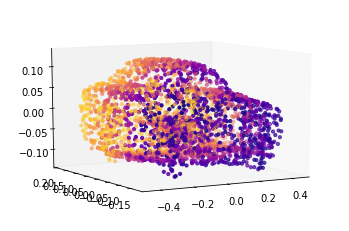
\includegraphics[width = 50mm]{car-shapenet-1} &
            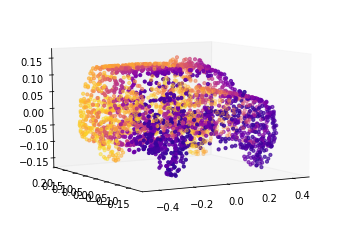
\includegraphics[width = 50mm]{car-shapenet-2} \\
        \end{tabular}
        \caption{Two car samples generated with ShapeNet.}
    \end{figure}


    \begin{figure}
        \centering
        \begin{tabular}{cc}
            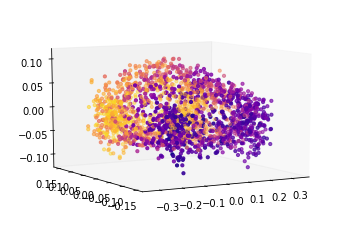
\includegraphics[width = 50mm]{car-lgan}
        \end{tabular}
        \caption{Car sample generated with l-GAN.}
    \end{figure}


    \begin{figure}
        \centering
        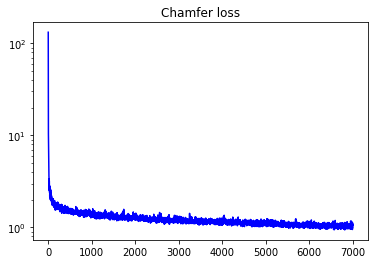
\includegraphics[width = 50mm]{chamfer-loss}
    \end{figure}


    \section{Challenges and Conclusions}
    \contentdescription{
        Challenges and Conclusions (5-15\%):
        Challenges you faced when reimplementing the paper and conducting the experiments.
        Were all details in the paper?
        Or did you have to look in the authors code or even contact them to find about some details?
        Was parts of the code quite hard to get them to work as intended?
        Did you have optimize and tune several hyperparameters?
        Which ones?
        Did the framework you used make the implementation difficult in some ways?

        Summarize your key results - what have you learned?
        What points do you think one should consider when using the approach of the paper you chose for your project?
        Suggest ideas for future extensions or new applications of your ideas.
    }

    One of the conclusions we arrived is that we were able to reproduce the results in~\cite{pmlr-v80-achlioptas18a}.

    The latent space GANs (l-GANs) was able to achieve better reconstructions.
    By contrast, the raw GAN performance is considerably lower when not enough data is provided.

    For example, in some of our experiments we found that the lamp data were insufficient to train the raw GAN reasonably well.


    \section{Ethical consideration, societal impact, potential alignment with UN SDGs}
    \contentdescription{
        Ethical consideration, societal impact, potential alignment with UN SDGs (5-10\%):
        Think and research!
        Are there any ethical considerations for the original paper, its problem or method, its way of conducting experiments?
        How about your task, your datasets, and the experiments you did?
        What societal impact can you imagine about the original paper and its contributions and results?
        How about your project report?
        How do you think this paper can push the UN SDG targets?
    }

    The Sustainable Development Goals (SDGs), were adopted by the United Nations in 2015 as a universal call
    to end poverty and protect the planet\footnote{\url{https://sdgs.un.org/goals}}, intended to be achieved by the year 2030.
    % For the sake of completeness, we mention the goals:
    % \begin{enumerate}
    %    \item No Poverty,
    %    \item Zero Hunger,
    %    \item Good Health and Well-being,
    %    \item Quality Education,
    %    \item Gender Equality,
    %    \item Clean Water and Sanitation,
    %    \item Affordable and Clean Energy,
    %    \item Decent Work and Economic Growth,
    %    \item Industry, Innovation and Infrastructure,
    %    \item Reducing Inequality,
    %    \item Sustainable Cities and Communities,
    %    \item Responsible Consumption and Production,
    %    \item Climate Action,
    %    \item Life Below Water,
    %    \item Life On Land,
    %    \item Peace, Justice, and Strong Institutions,
    %    \item Partnerships for the Goals.
    %\end{enumerate}

    Use of GANs can impact indirectly in all of the goals.
    However, we have chosen three items, which we consider the most directly affected:
    \textbf{Decent Work and Economic Growth}, \textbf{Industry, Innovation and Infrastructure}, and
    \textbf{Sustainable Cities and Communities}.

    We base our position on the fact ethical uses of machine learning can have a positive impact in societal development.
    Technology can leave humans in overseeing positions, avoiding dangerous or repetitive tasks.
    In addition, automation of processes, like the ones presented in this paper, can lead to a more efficient use of resources.

    GANs can also be used to deceive systems.
    The physical adversarial attack is analyzed by~\cite{arxiv:1812.10217} where they discuss
    how a system can be used to confuse face recognition in authentication and objection detection in autonomous driving cars.

    These systems like this one should be deployed only if the ethical stakeholders accept them.
    Especially, for a specific task, the first questions is: ``Should be use an AI system for that?''.

    We went the extra mile about the ethical consequences of AI and found how a major companies like Google\footnote{\url{https://ai.google/principles/}} faces this issue.
    The company explicitly stands state against use of AI in overall harm, weapons and other tools to kill or injure people, surveillance violating international norms, and contravention of principles in international law and human rights.



    \begin{ack}
        This work is partially supported by the Wallenberg AI, Autonomous Systems and Software Program (WASP) funded by the Knut and Alice Wallenberg Foundation.
    \end{ack}

    \bibliographystyle{plain}

    \bibliography{bibliography}

\end{document}

